\hypertarget{section-building-block-view}{%
\section{Building Block View}\label{section-building-block-view}}

\subsection{Level 1 - Context}\label{sub:5:l1}

EscapeDoom is developed with the intent to not create/maintain all parts it requires. Systems such as image hosting or the authentication provider are not part of the EscapeDoom software system, as can be seen in figure \ref{fig:c4:c1} below.

\begin{figure}
    \centering
    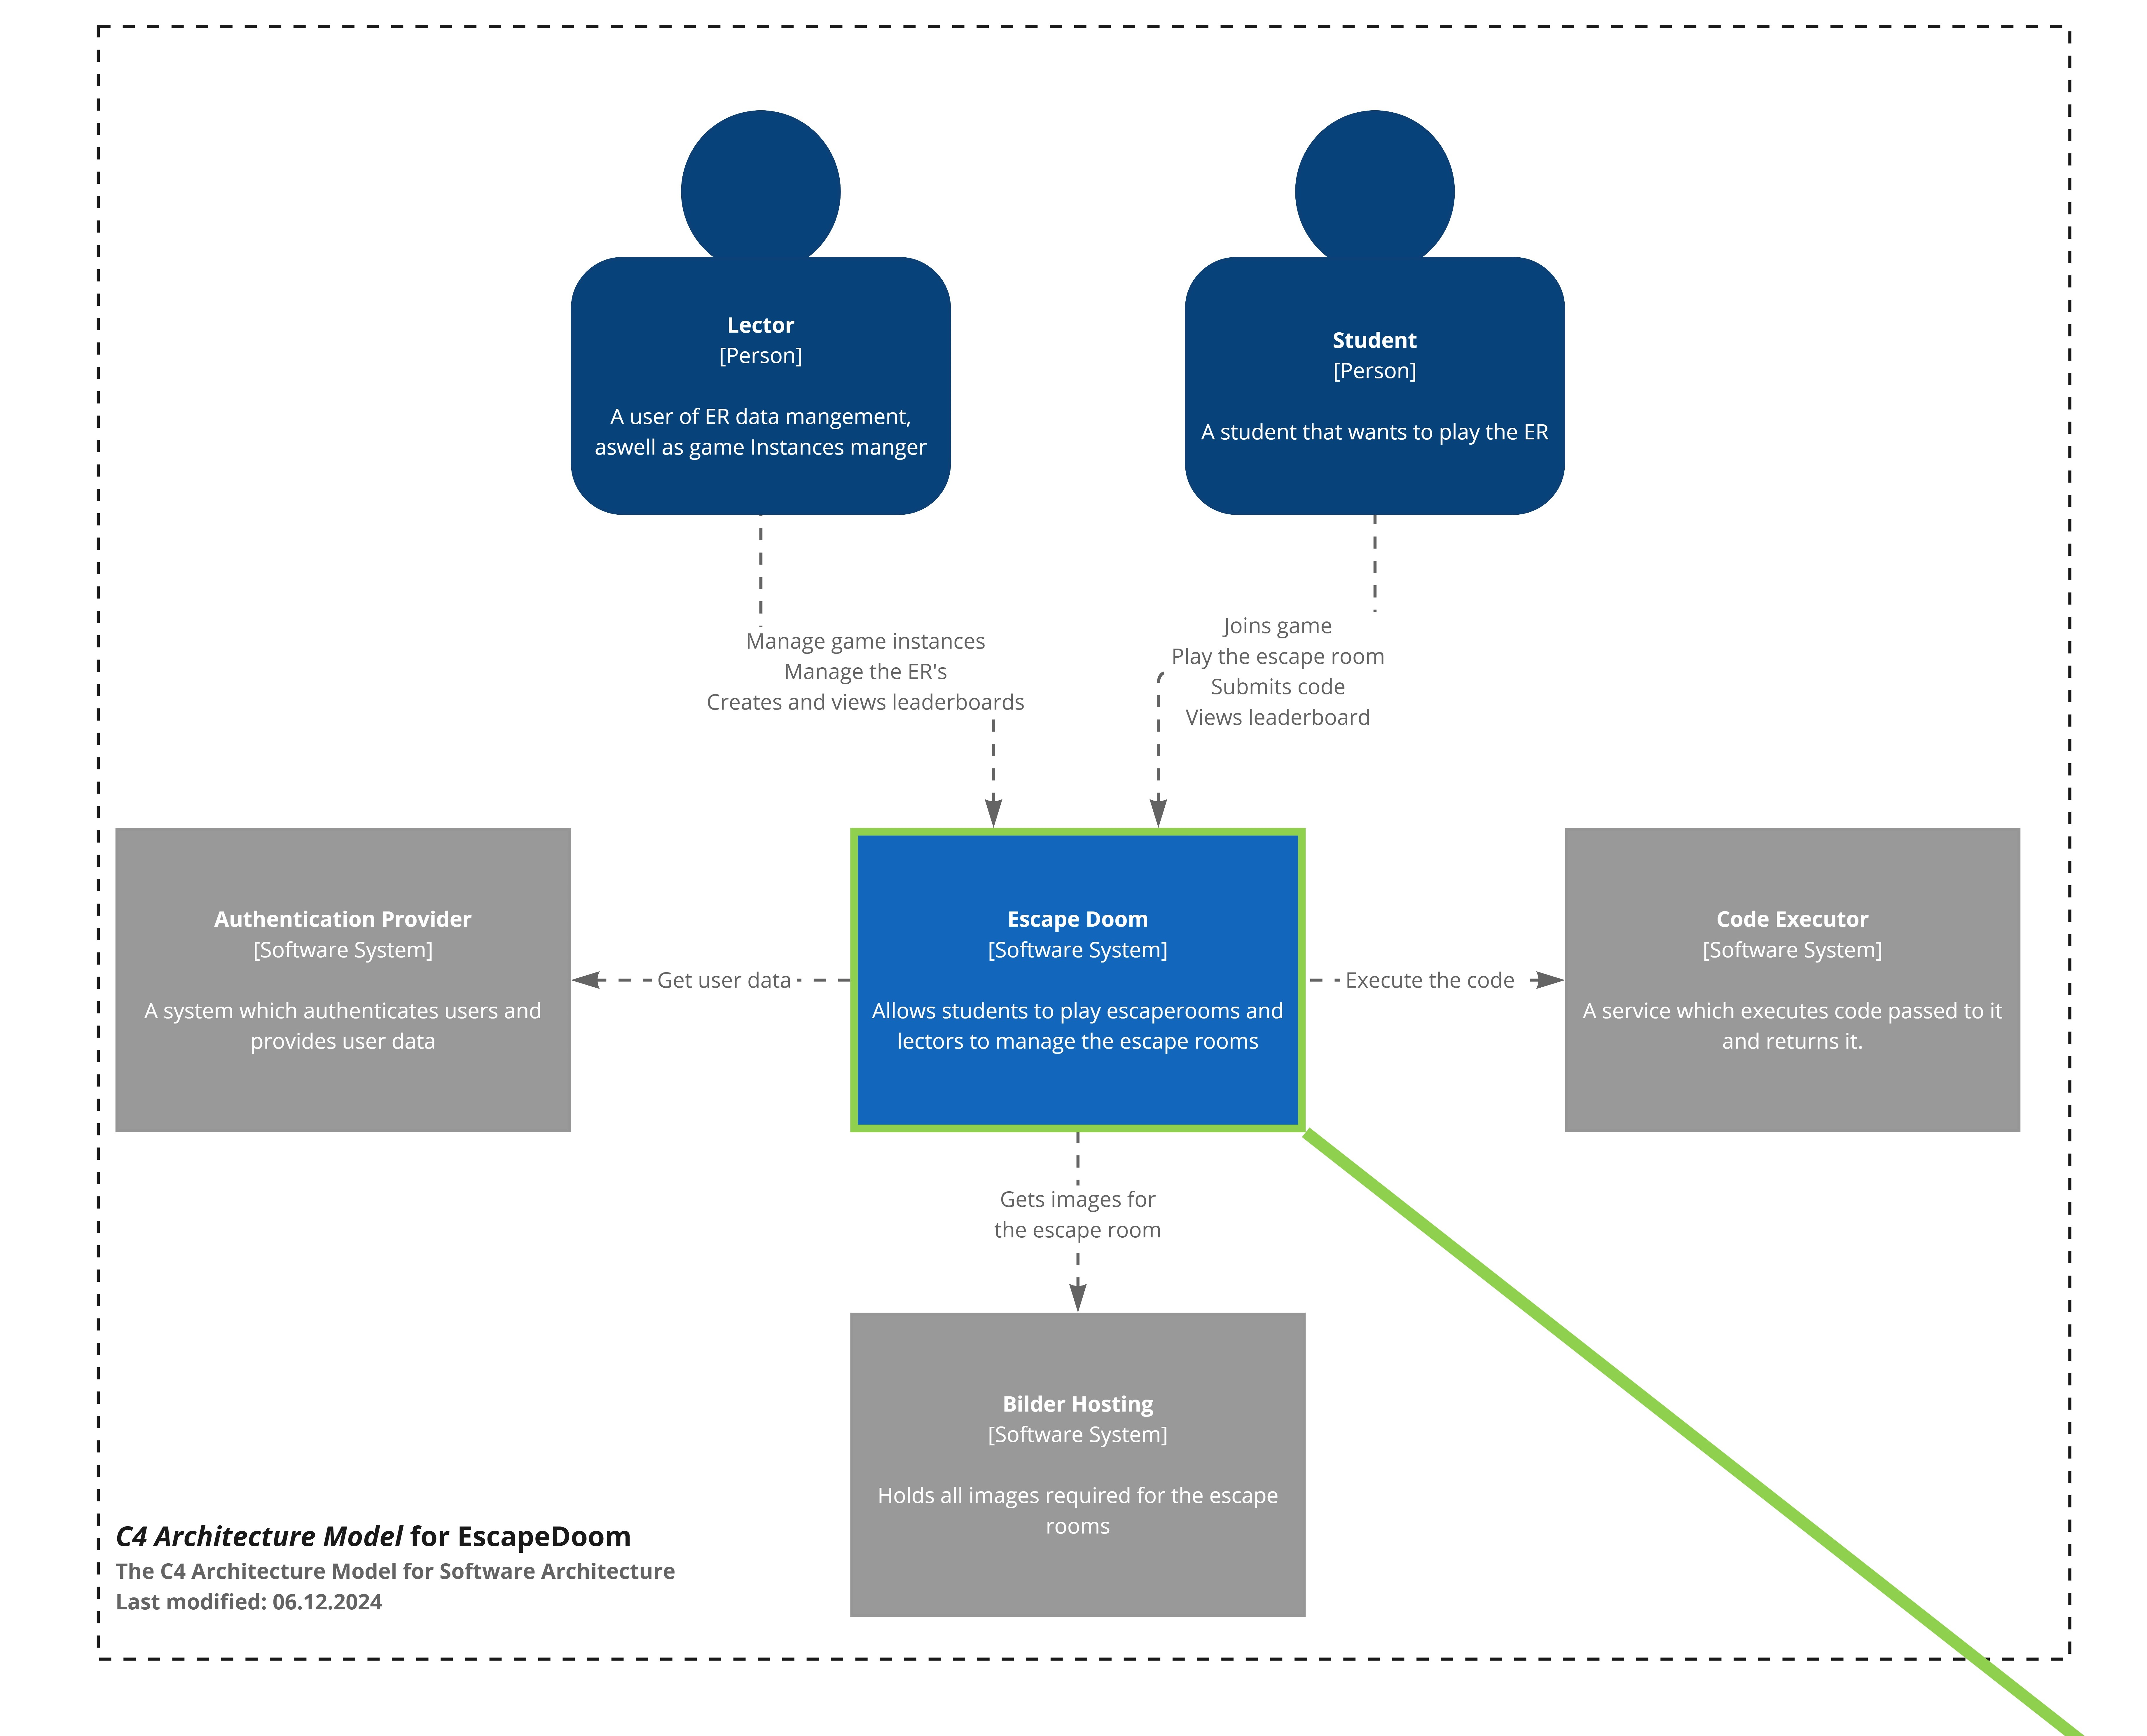
\includegraphics[width=1\linewidth]{images/C4/C1 - EscapeDoom.jpg}
    \caption{Level 1 - Escape Doom}
    \label{fig:c4:c1}
\end{figure}

\begin{table}[h!tbp]
    \centering
    \begin{tabularx}{1\textwidth} {
        | >{\raggedright\arraybackslash}X
        | >{\raggedleft\arraybackslash}X | }
        \hline
        Authentication Provider & Authenticates users to manage access \\
        \hline
        Escpae Doom & The main system, with which the lectors and students interact with \\
        \hline
        Code Executor & Responsible for executing code submitted by students \\
        \hline
        Bilder Hosting & Host images that are displayed in the escape rooms \\
        \hline
    \end{tabularx}
    \caption{Explanation of the individual blocks displayed in the Level 1 Context}
    \label{tab:c4:c1}
\end{table}

\newpage

\subsection{Level 2 - Containers}\label{sub:5:l2}

The EscapeDoom application itself can be segmented into multiple subsystems as depicted in \nameref{fig:c4:c2}. Each dotted line indicates communication, and thus a technical dependency. As can be seen, the front-end is maintained as one application while the back-end is split into microservices. The are then grouped into three separate domains as can be seen by the dotted lines.

\begin{figure}[h!tbp]
    \centering
    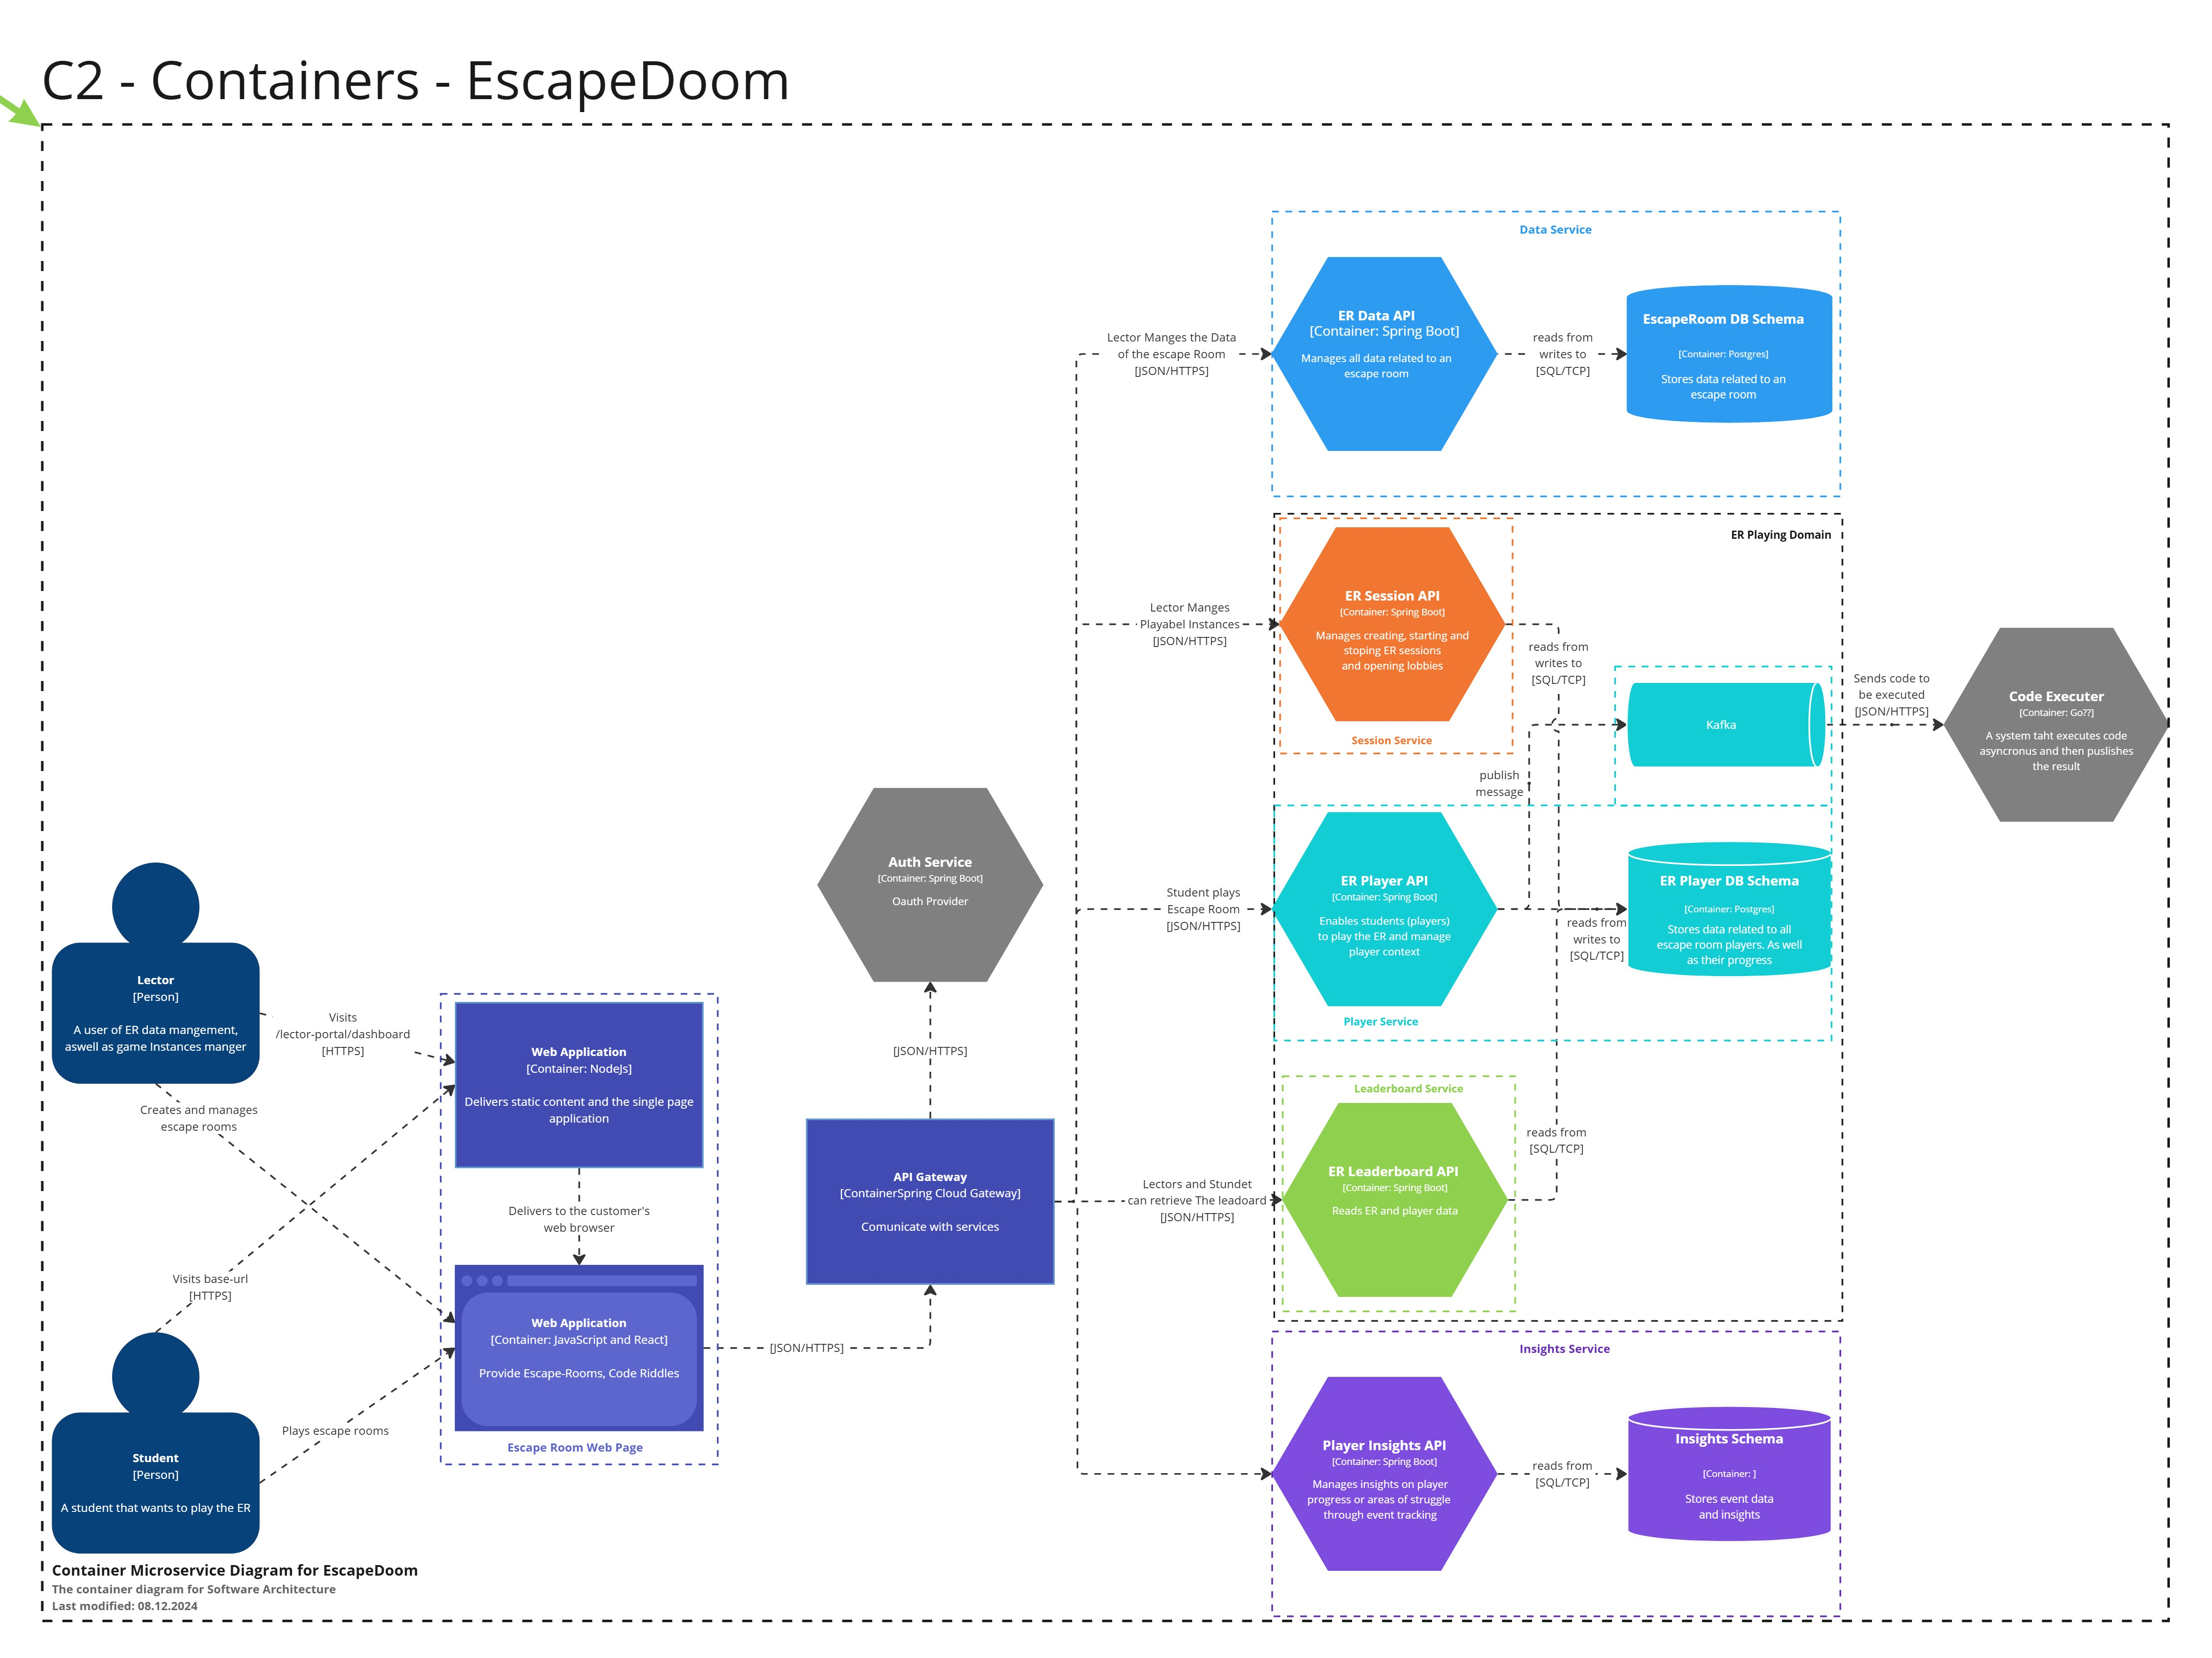
\includegraphics[width=0.9\linewidth]{images/C4/C2 - Containers.jpg}
    \caption{Level 2 - Containers}
    \label{fig:c4:c2}
\end{figure}

